\documentclass[handout,nooutcomes]{ximera}
%% handout
%% space
%% newpage
%% numbers
%% nooutcomes

%I added the commands here so that I would't have to keep looking them up
%\newcommand{\RR}{\mathbb R}
%\renewcommand{\d}{\,d}
%\newcommand{\dd}[2][]{\frac{d #1}{d #2}}
%\renewcommand{\l}{\ell}
%\newcommand{\ddx}{\frac{d}{dx}}
%\everymath{\displaystyle}
%\newcommand{\dfn}{\textbf}
%\newcommand{\eval}[1]{\bigg[ #1 \bigg]}

%\begin{image}
%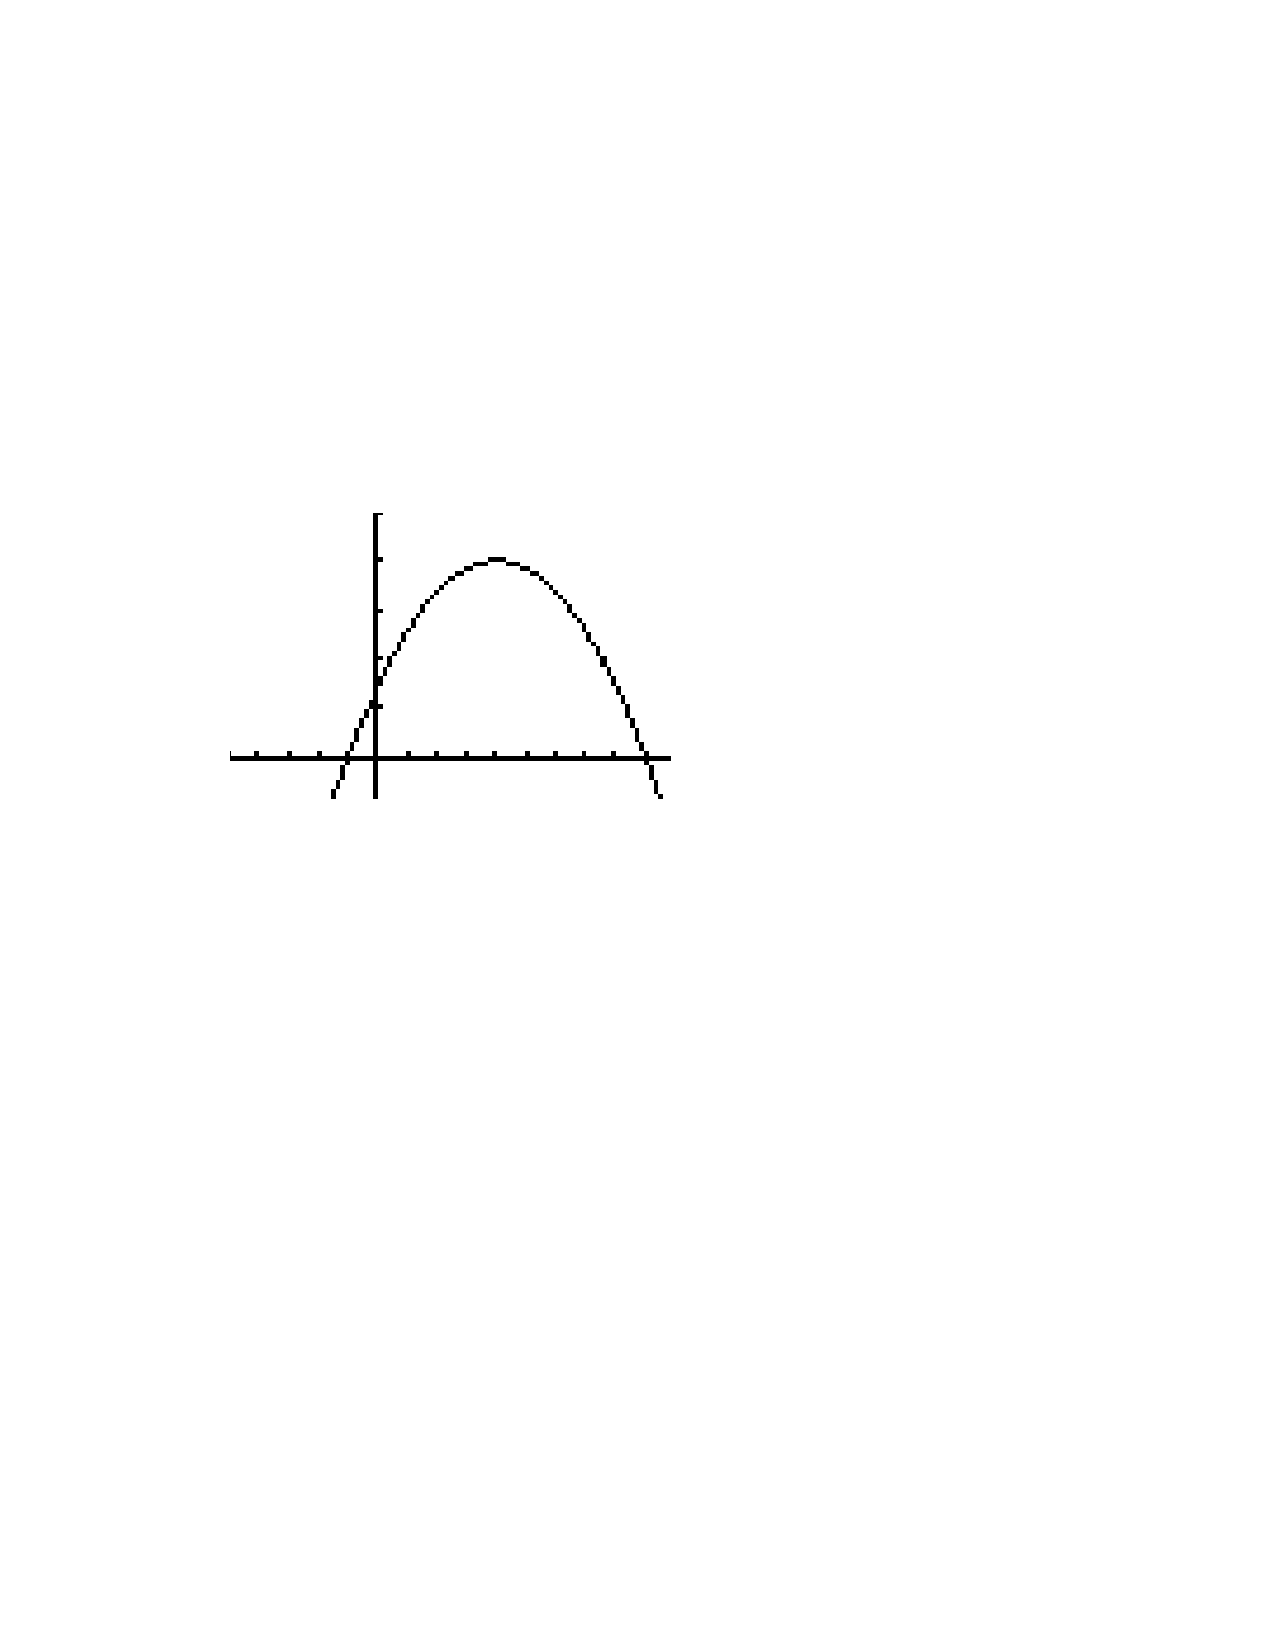
\includegraphics[trim= 170 420 250 180]{Figure1.pdf}
%\end{image}


\newcommand{\RR}{\mathbb R}
\renewcommand{\d}{\,d}
\newcommand{\dd}[2][]{\frac{d #1}{d #2}}
\renewcommand{\l}{\ell}
\newcommand{\ddx}{\frac{d}{dx}}
\newcommand{\dfn}{\textbf}
\newcommand{\eval}[1]{\bigg[ #1 \bigg]}

\usepackage{multicol}

\renewenvironment{freeResponse}{
\ifhandout\setbox0\vbox\bgroup\else
\begin{trivlist}\item[\hskip \labelsep\bfseries Solution:\hspace{2ex}]
\fi}
{\ifhandout\egroup\else
\end{trivlist}
\fi} %% we can turn off input when making a master document

\title{Recitation \#27 - 5.5 Substitution Rule}  

\begin{document}
\begin{abstract}		\end{abstract}
\maketitle

\section*{Warm up:} 
What are two substitutions that can be used to evaluate the integral
	\begin{equation*}
	\int x \sqrt{x+8} \d x
	\end{equation*}
	
		\begin{freeResponse}
		Two substitutions which work are $u=x+8$ and $v=\sqrt{x+8}$.  
		I find the $u=x+8$ to be the more ``obvious" solution, so let us work through that one first.
		\begin{equation*}
		u=x+8 \quad \Longrightarrow \quad \d u = \d x \quad \text{and} \quad x = u-8
		\end{equation*}
		Substituting into the original integral and solving:
		\begin{align*}
		\int x \sqrt{x+8} \d x &= \int (u-8) \sqrt{u} \d u  \\
		&= \int (u^{\frac{3}{2}} - 8u^{\frac{1}{2}} ) \d u  \\
		&= \frac{2}{5} u^{\frac{5}{2}} - 8 \cdot \frac{2}{3} u^{\frac{3}{2}} + C  \\
		&= \frac{2}{5} (x+8)^{\frac{5}{2}} - \frac{16}{3} (x+8)^{\frac{3}{2}} + C
		\end{align*}
		
		To the other solution, letting $v=\sqrt{x+8}$ gives:
		\begin{equation*}
		\d v = \frac{1}{2 \sqrt{x+8}} \d x = \frac{1}{2v} \d x 	\quad	\Longrightarrow \quad \d x = 2v \d v
		\end{equation*}
		and
		\begin{equation*}
		v = \sqrt{x+8} \quad \Longrightarrow \quad v^2 = x+8 \quad \Longrightarrow \quad x= v^2-8
		\end{equation*}
		Substituting into the original integral and solving:
		\begin{align*}
		\int x \sqrt{x+8} \d x &= \int (v^2-8)(v)(2v)\d v  \\
		&= \int (2v^4 - 16v^2) \d v  \\
		&= \frac{2}{5} v^5 - \frac{16}{3} v^3 + C  \\
		&= \frac{2}{5} (\sqrt{x+8})^5 - \frac{16}{3} (\sqrt{x+8})^3 + C
		\end{align*}
		
		\end{freeResponse}	
		
		
		

	
	
	
	
	

\section*{Group work:}
















%problem 2
\begin{problem}
Compute the following integrals:

	\begin{enumerate}
	
	%part a
	\item  $\int \cos(x) \sqrt{\sin(x)} \d x$
		\begin{freeResponse}
		Let $v = \sin(x)$.  Then $\d v = \cos(x) \d x$, and so
			\begin{align*}
			\int \cos(x) \sqrt{\sin(x)} \d x &= \int \sqrt{v} \d v  \\
			&= \frac{2}{3} v^{\frac{3}{2}} + C  \\
			&= \frac{2}{3} (\sin(x))^{\frac{3}{2}} + C.
			\end{align*}
		\end{freeResponse}
		
		
		
	%part b
	\item  $\int \left( 3t^2 - 4 + \frac{1}{t} \right) e^{t^3 - 4t + \ln(t) - 9} \d t$
		\begin{freeResponse}
		This problem looks a lot more difficult than it really is.  Let $w=t^3 - 4t + \ln(t) - 9$.  
		Then $\d w = \left( 3t^2 - 4 + \frac{1}{t} \right) \d t$.  But this is exactly the coefficient of the exponential term in the integral.  So
			\begin{align*}
			\int \left( 3t^2 - 4 + \frac{1}{t} \right) e^{t^3 - 4t + \ln(t) - 9} \d t &= \int e^w \d w  \\
			&= e^w + C  \\
			&= e^{t^3 - 4t + \ln(t) - 9} + C.
			\end{align*}
		\end{freeResponse}
		
		
		
	\end{enumerate}
		
		
		

\end{problem}
	
	
	
	
	












%problem 4
\begin{problem}
Evaluate the following integrals:

	\begin{enumerate}
	
	%part a
	\item  $\int_{-2}^1 t^2 \sin(t^3) \d t$
		\begin{freeResponse}
		Let $u=u(t) = t^3$, where $``u(t)"$ is just meant to indicate that the variable $u$ is really a function of $t$.  Then $\d u = 3t^2 \d t$.  But also notice that
			\begin{align*}
			u(-2) &= (-2)^3 = -8  \\
			u(1) &= 1^3 = 1
			\end{align*}
		Then
			\begin{align*}
			\int_{-2}^1 t^2 \sin(t^3) \d t &= \frac{1}{3} \int_{-2}^1 3 t^2 \sin(t^3) \d t  \\
			&= \frac{1}{3} \int_{-8}^1 \sin(u) \d u  \\
			&= - \frac{1}{3} \eval{\cos(u)}_{-8}^1  \\
			&= - \frac{1}{3} ( \cos(1) - \cos(-8)).
			\end{align*}
		\end{freeResponse}
		
		
		
	%part b
	\item  $\int_0^{\frac{1}{2}} \frac{13e^x}{3e^x - 5} \d x$
		\begin{freeResponse}
		Let $v=3e^x - 5$.  Then
			\begin{align*}
			&\d v = 3e^x \d x  \\
			&v(0) = 3e^0 -5= 3-5=-2  \\
			&v\left( \frac{1}{2} \right) = 3e^{\frac{1}{2}} - 5.
			\end{align*}
		So
			\begin{align*}
			\int_0^{\frac{1}{2}} \frac{13e^x}{3e^x - 5} \d x &= \frac{13}{3} \int_0^{\frac{1}{2}} \frac{3e^x}{3e^x - 5} \d x  \\
			&= \frac{13}{3} \int_{-2}^{3e^{\frac{1}{2}}-5} \frac{1}{v} \d v  \\
			&= \frac{13}{3} \eval{\ln|v|}_{-2}^{3e^{\frac{1}{2}}-5}  \\
			&= \frac{13}{3} \left( \ln|3e^{\frac{1}{2}}-5| - \ln|-2| \right).  \\
			\end{align*}
		\end{freeResponse}
		
		
		
	\end{enumerate}
			
			
	
\end{problem}







%problem 5
\begin{problem}
Evaluate the following integrals:

	\begin{enumerate}
	
	%part a
	\item  $\int_1^4 \frac{e^{\sqrt{x}}}{3\sqrt{x}} \d x$
		\begin{freeResponse}
		Let $w=\sqrt{x}$.  Then
			\begin{align*}
			&\d w = \frac{1}{2 \sqrt{x}} \d x  \\
			&w(1) = \sqrt{1} = 1  \\
			&w(4) = \sqrt{4} = 2.
			\end{align*}
		So
			\begin{align*}
			\int_1^4 \frac{e^{\sqrt{x}}}{3\sqrt{x}} \d x &= \frac{2}{3} \int_1^4 \frac{e^{\sqrt{x}}}{2\sqrt{x}} \d x  \\
			&= \frac{2}{3} \int_1^2 e^w \d w  \\
			&= \frac{2}{3} \eval{e^w}_1^2  \\
			&= \frac{2}{3} (e^2 - e).
			\end{align*}
		\end{freeResponse}
		
		
		
	%part b
	\item  $\int_{\frac{\pi}{3}}^{\frac{\pi}{2}} \sin(x) \sec^2(\cos(x)) \d x$
		\begin{freeResponse}
		Let $u=\cos(x)$.  Then
			\begin{align*}
			&\d u = -\sin(x) \d x  \\
			&u\left( \frac{\pi}{3} \right) = \frac{1}{2}  \\
			&u\left( \frac{\pi}{2} \right) = 0.
			\end{align*}
		So
			\begin{align*}
			\int_{\frac{\pi}{3}}^{\frac{\pi}{2}} \sin(x) \sec^2(\cos(x)) \d x &= - \int_{\frac{1}{2}}^0 \sec^2(u) \d u   \\
			&= - \eval{\tan(u)}_{\frac{1}{2}}^0  \\
			&=  -\left( 0 - \tan\left( \frac{1}{2} \right) \right)  \\
			&= \tan \left( \frac{1}{2} \right).
			\end{align*}
		\end{freeResponse}
		
		
		
	\end{enumerate}
			
			
	
\end{problem}







\newpage
\begin{center}
\begin{large}
{\bf  Additional Practice Problems}
\end{large}
\end{center}







%problem 1
\begin{problem}
Compute the following integrals:

	\begin{multicols}{2}
	\begin{enumerate}
	
	%part a
	\item  $\int 2t \sin \left( t^2 \right) \d t$
		\begin{freeResponse}
		Let $w=t^2$.  Then $\d w = 2t \d t$, and so
			\begin{align*}
			\int 2t \sin(t^2) \d t &= \int \sin(w) \d w  \\
			&= - \cos(w) + C  \\
			&= - \cos(t^2) + C.
			\end{align*}
		\end{freeResponse}
		
		
		
	%part b
	\item  $\int \sec^2(x) \tan(x) \d x$
		\begin{freeResponse}
		Let $u = \tan(x)$.  Then $\d u = \sec^2 (x) \d x$, and so
			\begin{align*}
			\int \sec^2(x) \tan(x) \d x &= \int u \d u  \\
			&= \frac{1}{2} u^2 + C  \\
			&= \frac{1}{2} \tan^2(x) + C.
			\end{align*}
		Note that the substitution $v=\sec(x)$ would also work to solve this problem.  
		It is a good exercise to work this out!
		\end{freeResponse}
		

	
	%part a
	\item  $\int \frac{x^2 }{1 + x^2} \d x$
		\begin{freeResponse}
		In general, when integrating a rational function where the degree of the numerator is greater than or equal to the degree
		of the denominator, you want to do long division to get the smallest possible degree in the numerator.  
		But watch this slick little trick:
			\begin{equation*}
			\frac{x^2}{1+x^2} = \frac{1 + x^2 - 1}{1+x^2} = \frac{1+x^2}{1+x^2} - \frac{1}{1+x^2} = 1 - \frac{1}{1+x^2}.
			\end{equation*}
		So
			\begin{align*}
			\int \frac{x^2 }{1 + x^2} \d x &= \int \left( 1 - \frac{1}{1+x^2} \right) \d x  \\
			&= x - \arctan(x) + C.
			\end{align*}
		I learned the trick above through tons and tons of practice solving integrals.  
		So guess what is a good idea for you to do before the final exam???
		\end{freeResponse}
		
		
		
	%part b
	\item  $ \int \frac{1+3x}{4+4x^2} \d x$
		\begin{freeResponse}
		First notice that
			\begin{equation*}
			\int \frac{1+3x}{4+4x^2} \d x = \frac{1}{4} \int \frac{1+3x}{1+x^2} \d x = \frac{1}{4} \int \left( \frac{1}{1+x^2} + \frac{3x}{1+x^2} \right) \d x.
			\end{equation*}
		The first integral is $\arctan(x)$, and so we have
			\begin{equation}\label{3b1}
			\int \frac{1+3x}{4+4x^2} \d x = \frac{1}{4} \arctan(x) + \frac{3}{4} \int \frac{x}{1+x^2} \d x.
			\end{equation}
		We can solve this second integral by substitution.  Let $u=1+x^2$.  Then $\d u = 2x \d x$ and $\frac{1}{2} \d u = x \d x$.  So
			\begin{equation}\label{3b2}
			\int \frac{x}{1+x^2} \d x = \frac{1}{2} \int \frac{1}{u} \d u = \frac{1}{2} \ln|u| +C = \frac{1}{2} \ln(1+x^2) + C.
			\end{equation}
		Plugging equation \eqref{3b2} into equation \eqref{3b1} yields
			\begin{equation*}
			\int \frac{1+3x}{4+4x^2} \d x = \frac{1}{4} \arctan(x) + \frac{3}{8} \ln(1+x^2) + C.
			\end{equation*}
		\end{freeResponse}
		
		
	
	%part a
	\item  $\int \frac{13x^7}{\sqrt{3x^4-5}} \d x$
		\begin{freeResponse}
		Let $v = 3x^4 - 5$.  Then
			\begin{align*}
			&\d v = 12 x^3 \d x  \\
			&x^4 = \frac{1}{3} (v + 5).
			\end{align*}
		So
			\begin{align*}
			\int \frac{13x^7}{\sqrt{3x^4-5}} \d x &= \frac{13}{12} \int \frac{(x^4)(12 x^3)}{\sqrt{3x^4-5}} \d x  \\
			&= \frac{13}{12} \int \frac{\frac{1}{3} (v+5)}{\sqrt{v}} \d v  \\
			&= \frac{13}{36} \int \left( v^{\frac{1}{2}} + 5v^{-\frac{1}{2}} \right) \d v  \\
			&= \frac{13}{36} \left( \frac{2}{3} v^{\frac{3}{2}} + 10 v^{\frac{1}{2}} \right) + C  \\
			&= \frac{13}{54} (3x^4-5)^{\frac{3}{2}} + \frac{65}{18} \sqrt{3x^4 - 5} + C.
			\end{align*}
		\end{freeResponse}
		
		
		
	%part b
	\item  $\int \frac{x^3}{x^2 - 3} \d x$
		\begin{freeResponse}
		Let $w = x^2 - 3$.  Then
			\begin{align*}
			&\d w = 2x \d x  \\
			&x^2 = w + 3.
			\end{align*}
		So
			\begin{align*}
			\int \frac{x^3}{x^2 - 3} \d x &= \frac{1}{2} \int \frac{(x^2)(2x)}{x^2 - 3} \d x  \\
			&= \frac{1}{2} \int \frac{w+3}{w} \d w  \\
			&= \frac{1}{2} \int \left(1 + \frac{3}{w} \right) \d w  \\
			&= \frac{1}{2} \left( w + 3 \ln|w| \right) + C  \\
			&= \frac{1}{2} \left( x^2 - 3 + 3\ln|x^2-3| \right) + C.
			\end{align*}
		\end{freeResponse}
		
		
		
	\end{enumerate}
	\end{multicols}
			
			
	
\end{problem}







%problem 7
\begin{problem}
Find the error in the following ``solution":

Find $\int_{-2}^2 \frac{1}{x^8 - 1} \d x$

	\begin{image}
	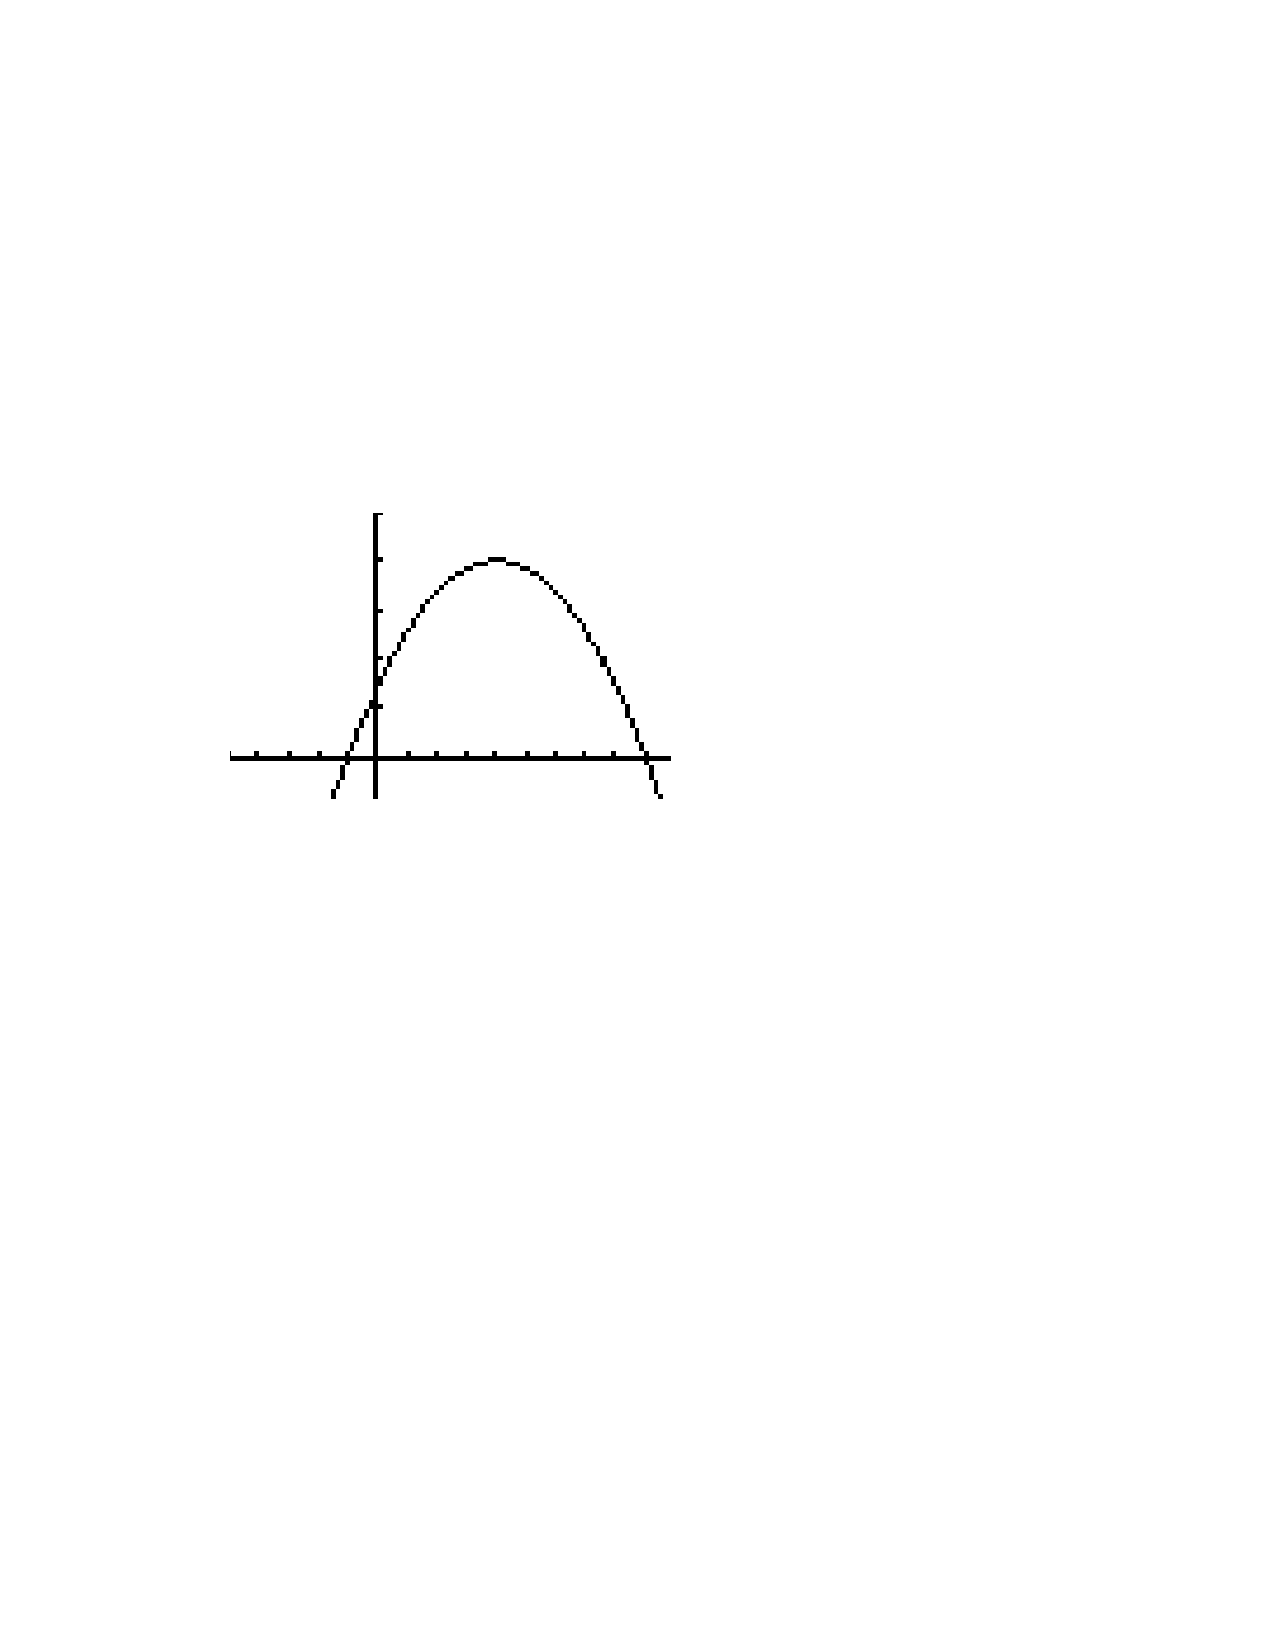
\includegraphics[trim= 120 320 350 180]{Figure1.pdf}
	\end{image}

	\begin{freeResponse}
	The error is that the function $\frac{1}{x^8-1}$ is not defined at $x=1$, and is therefore not continuous on the interval $[-2,2]$.
	\end{freeResponse}

\end{problem}








	
	
	
	
	
	
	
	
	

	










								
				
				
	














\end{document} 


















